\documentclass[12pt,a4paper]{article}
\usepackage{graphicx}

\begin{document}

\title{Description of master thesis}
\author{Morten Bendiksen}
\date{Mars 2011}
\maketitle

\section*{Rapid modeling of geological structures}


Geologist often make sketches of geological structures, both in order to communicate ideas amongst themselves, and to other interested people. We propose to develop a computer program to aid in this sketching.

In developing this program, the following techniques will be explored:
\begin{itemize}
 \item Having an initial empty sandbox from which the structures can be ``carved''
 \item Drawing layers by turning and sketching on the sides of the box
    \begin{itemize}
     \item Constraints on drawing. No layer-/self-intersection
     \item Layers will be interpolated from this
     \item Modifying layers by sketching on them and pushing or pulling
    \end{itemize}
 \item Drawing rivers by sketching on the surface of horizons
    \begin{itemize}
     \item Will carve out a plausible river following this path
     \item Allows adjustments of size and depth
     \item Adjusting of sealeves determines deposits
    \end{itemize}
  \item Drawing ridges and valleys
    \begin{itemize}
     \item Drawing the path of the new feature on existing terrain
     \item Adjust look of contour along this path
     \item Possibly change the height by similar approach as in Teddy
    \end{itemize}
\item Picking layers with mouse pointer
    \begin{itemize}
     \item Further editing of layer is then possible
     \item Changing color
     \item Setting tranparency
    \end{itemize}
\item Expanding sketch with new cubes
    \begin{itemize}
     \item Drawing layers in the new cube might use the edges of layers in adjacent cube
     \item While drawing lines will snap to existing lines
    \end{itemize}
\item Representations
    \begin{itemize}
     \item The terrain features will be modeled and stored by some sort of implisit representation
     \item Might be possible to go back and forth in the history of this structure to make changes withouth loosing later work
    \end{itemize}
\item Procedural geologic modeling
    \begin{itemize}
     \item Generate deposits by specifying terrain and sea level and such
     \item Changes to the generated structures might change the initial conditions needed to make such an end result
    \end{itemize}
\item Visualization options
    \begin{itemize}
     \item Generating simulations of seismic data
\end{itemize}


\section*{Illustrations of use case}
Here we show a possible sequence of manipulations to  quickly create some geological structures in a scene.
\begin{figure}
\centering
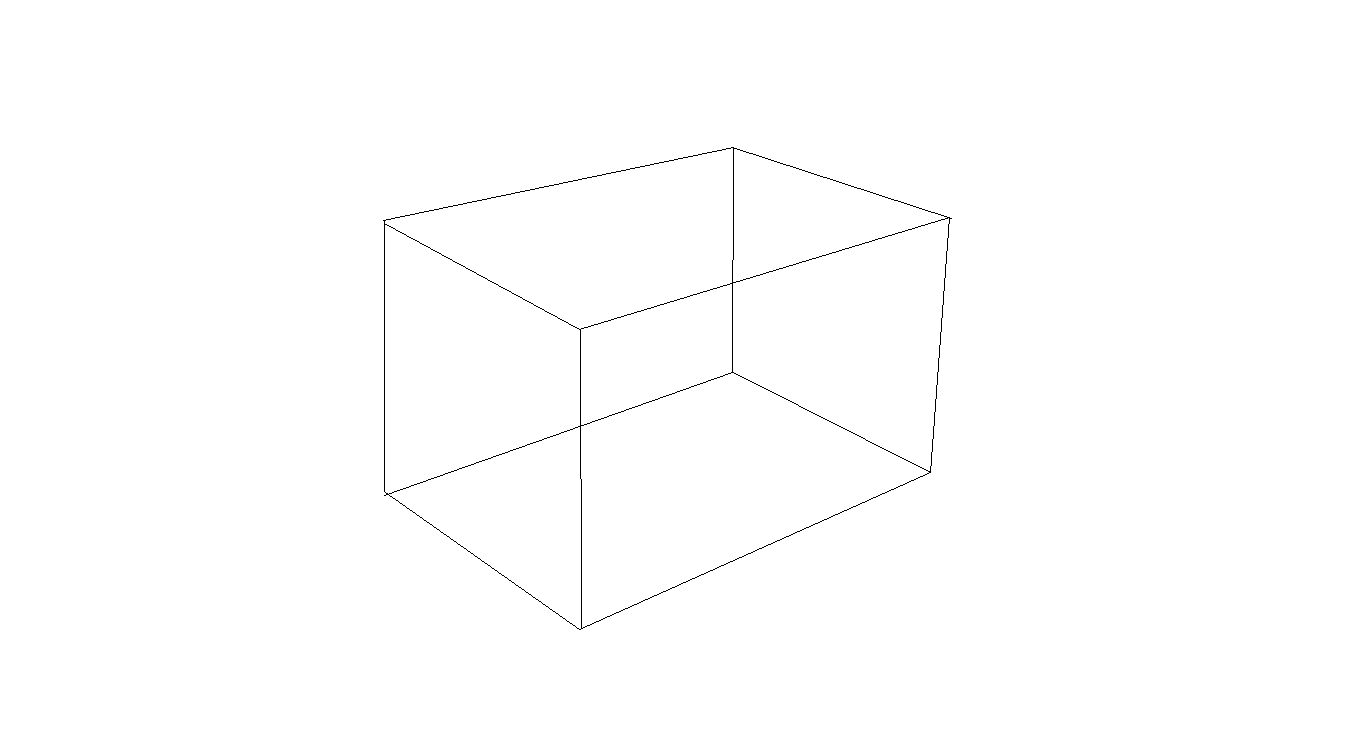
\includegraphics[width=4in]{box}
\caption[]{
  \footnotesize
  We start with the empty box
  \label{fig:box}
}
\end{figure}

\begin{figure}
\centering
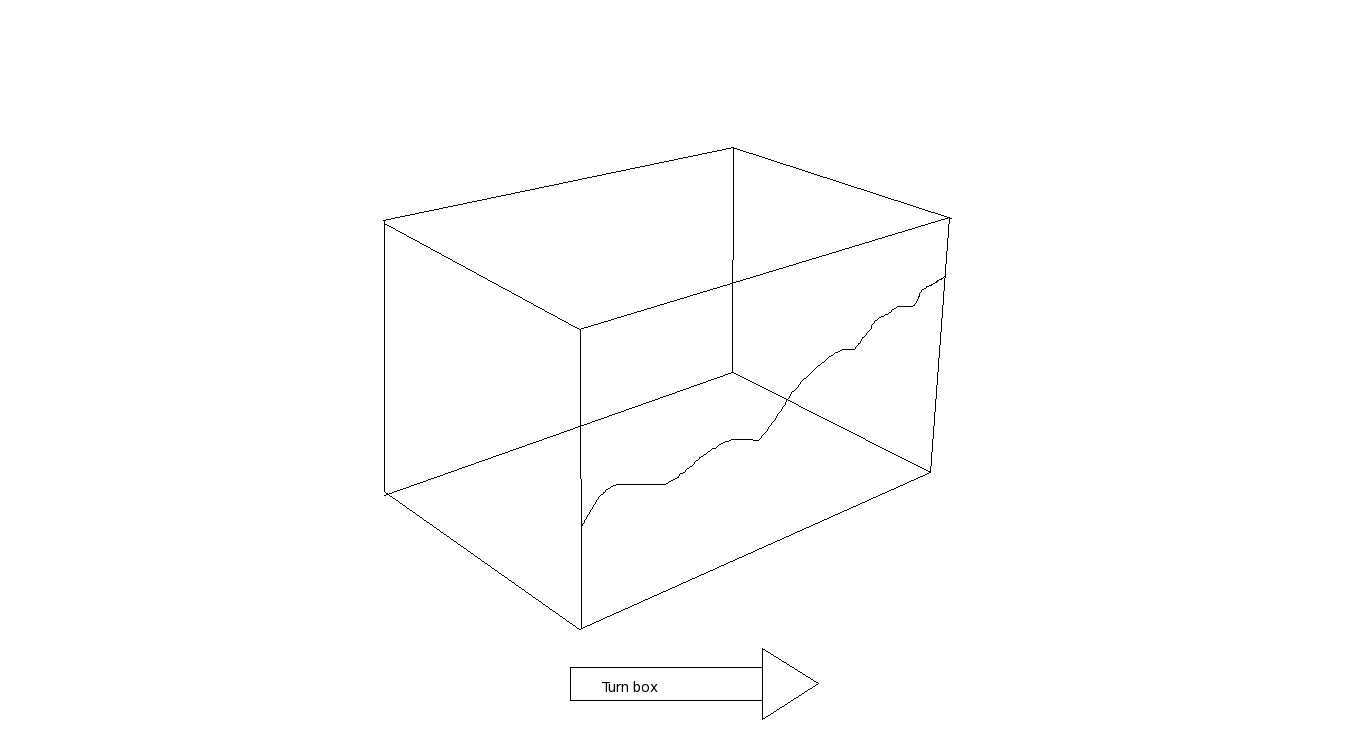
\includegraphics[width=4in]{turnBox}
\caption[]{
  \footnotesize
  We draw the imagined layer in the box by turning it and drawing on the sides
  \label{fig:turnBox}
}
\end{figure}

\begin{figure}
\centering
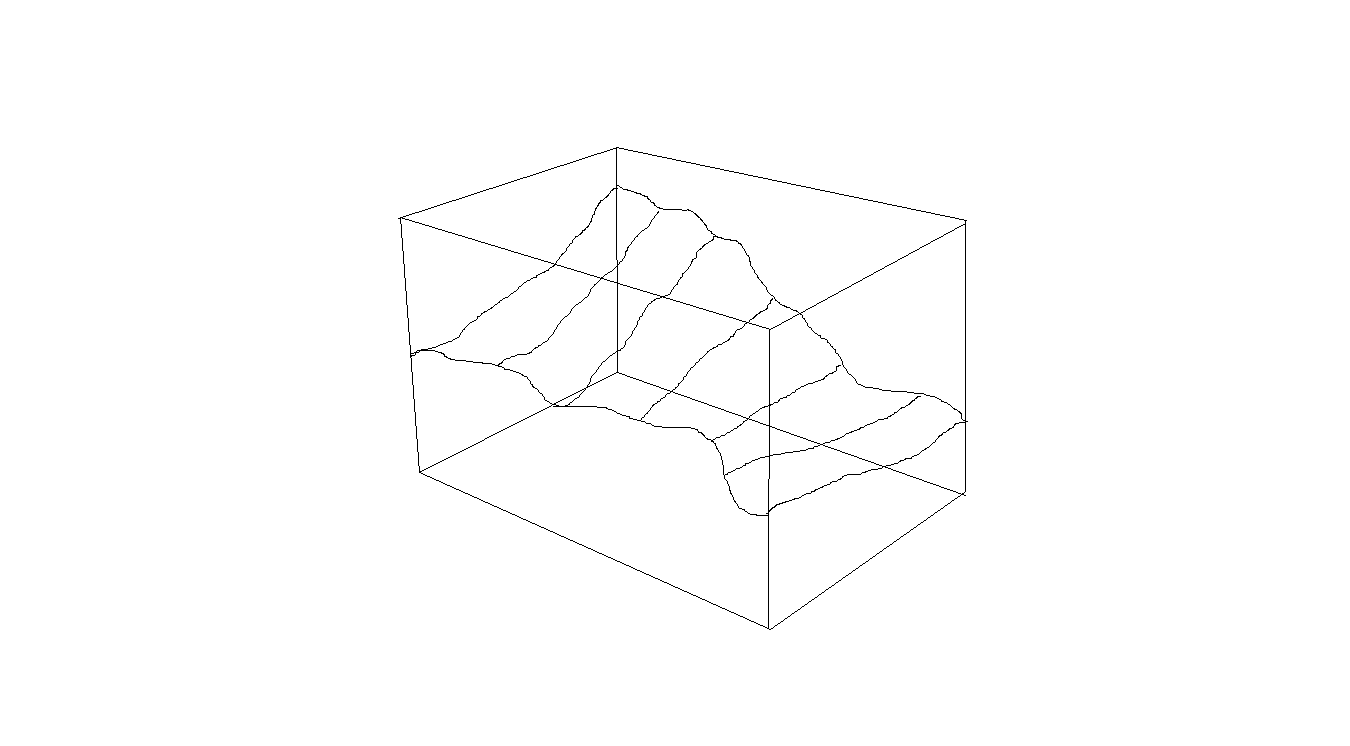
\includegraphics[width=4in]{interpolateLayer}
\caption[]{
  \footnotesize
  A layer is interpolated from the four sides we draw
  \label{fig:interpolateLayer}
}
\end{figure}

\begin{figure}
\centering
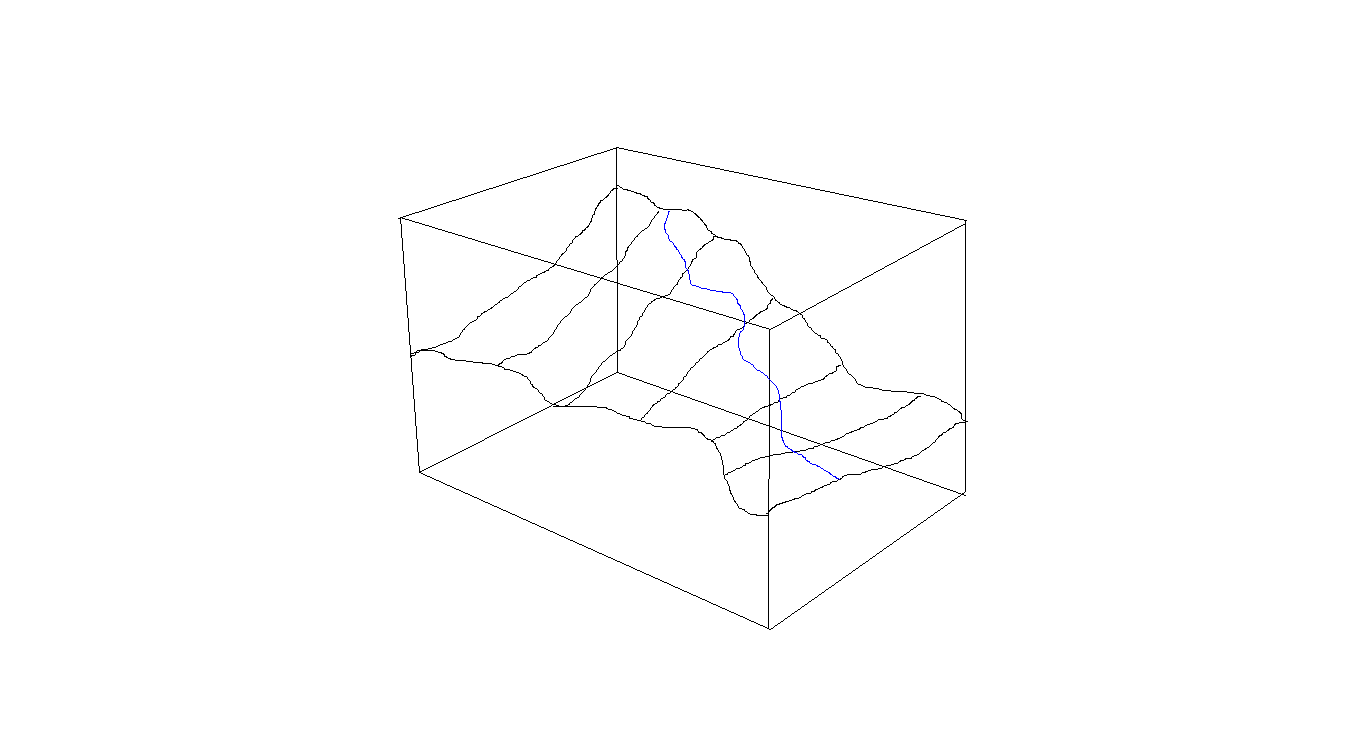
\includegraphics[width=4in]{drawRiver}
\caption[]{
  \footnotesize
  We draw a river path on this layer
  \label{fig:drawRiver}
}
\end{figure}

\begin{figure}
\centering
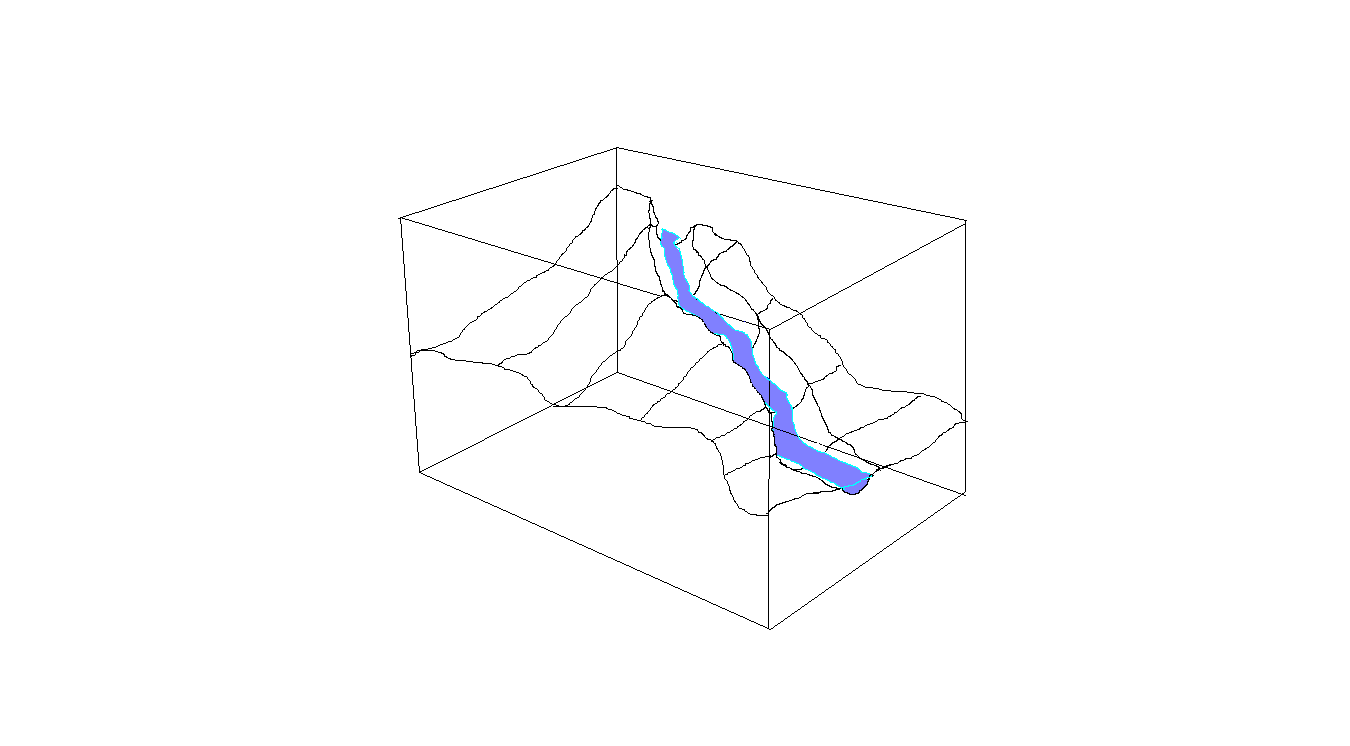
\includegraphics[width=4in]{carveRiver}
\caption[]{
  \footnotesize
  The computer will carve out from this layer as needed to make a river follow this path in a plausible way
  \label{fig:carveRiver}
}
\end{figure}

\begin{figure}
\centering
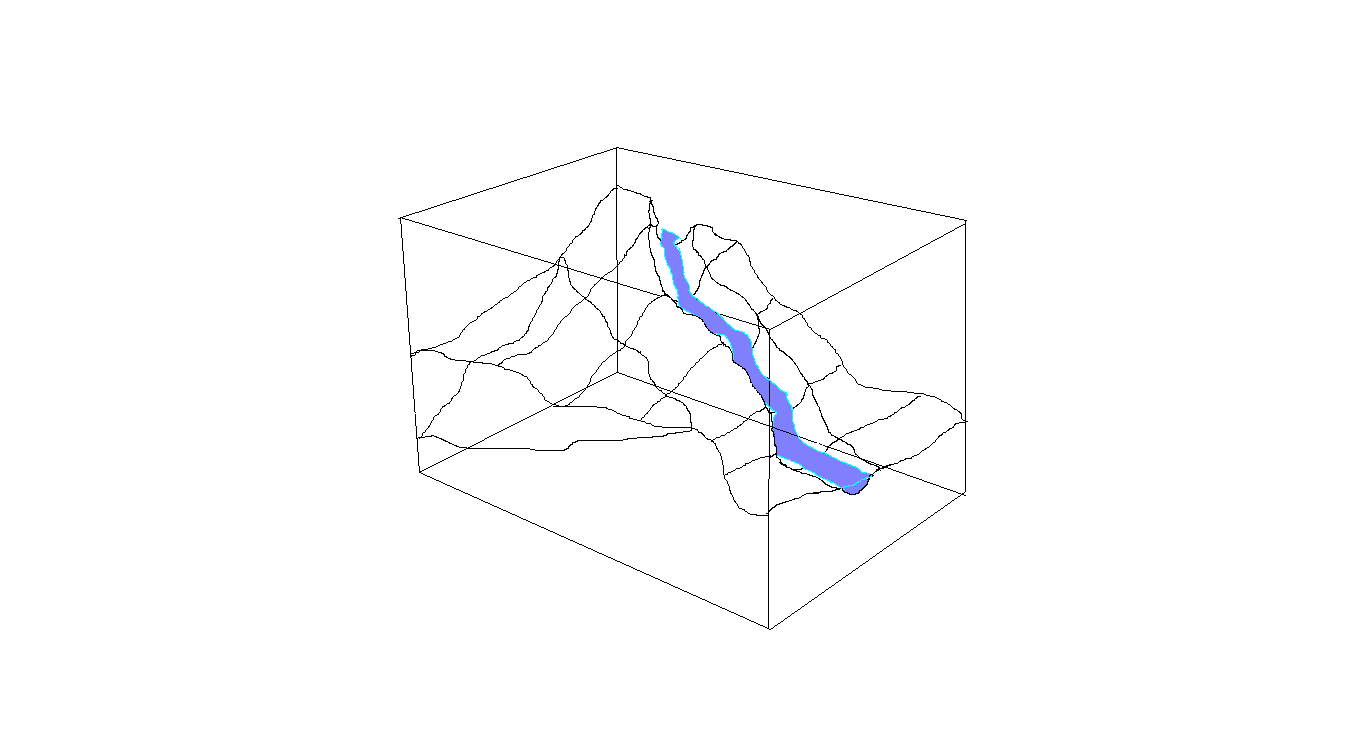
\includegraphics[width=4in]{drawNewLayer}
\caption[]{
  \footnotesize
  Now we draw a new layer. This can use the previous layer as a drawing surface in stead of only the sides of the box
  \label{fig:drawNewLayer}
}
\end{figure}

\begin{figure}
\centering
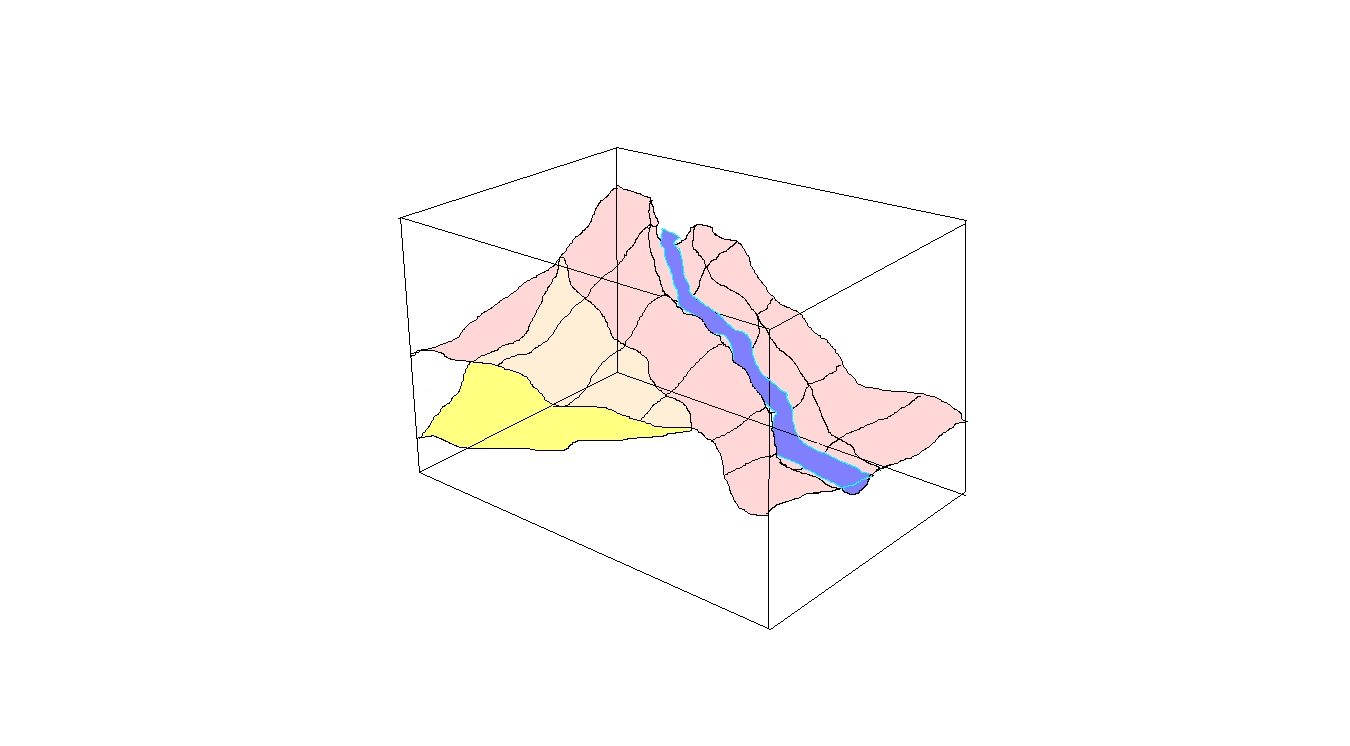
\includegraphics[width=4in]{addColor}
\caption[]{
  \footnotesize
  We add some color to the layers. In this figure the layers are partially transparent.
  \label{fig:addColor}
}
\end{figure}

\begin{figure}
\centering
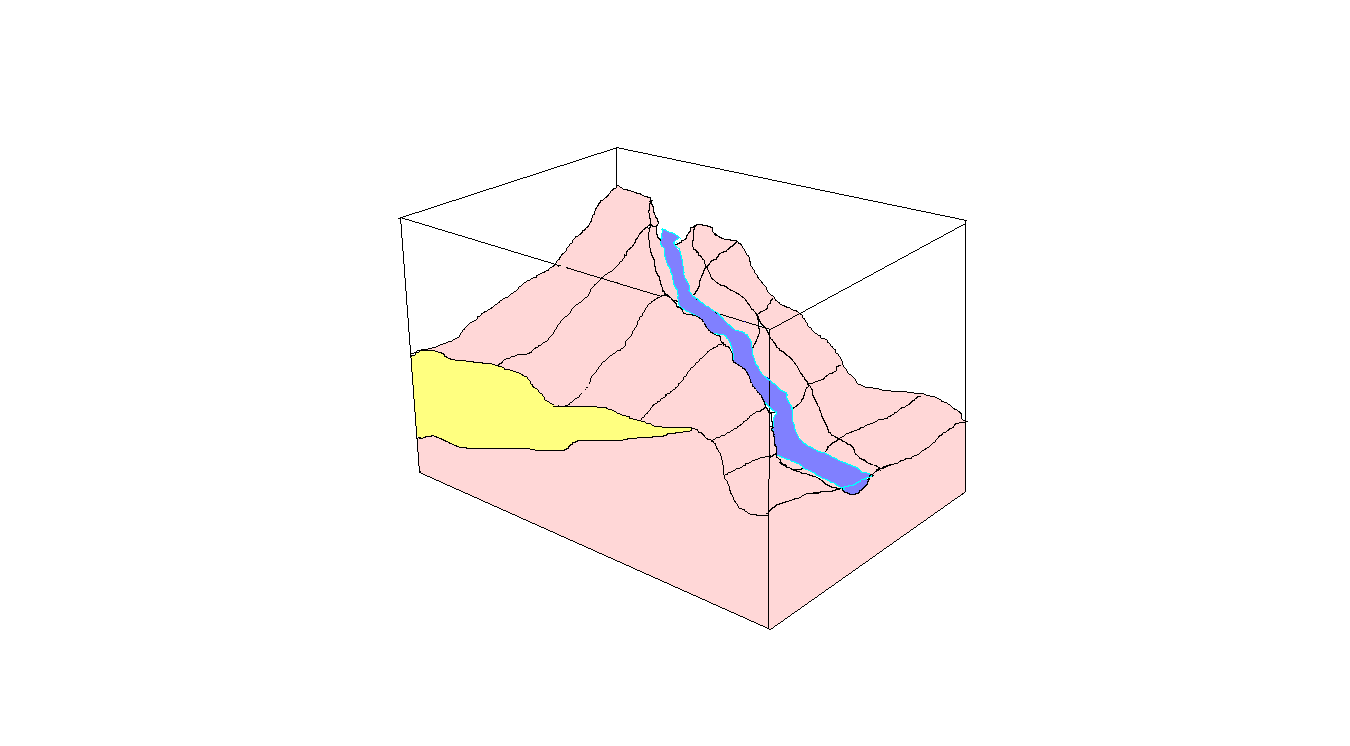
\includegraphics[width=4in]{offTransparency}
\caption[]{
  \footnotesize
  Here we have turned of tranparency and the sides become opaque
  \label{fig:offTransparency}
}
\end{figure}

\begin{figure}
\centering
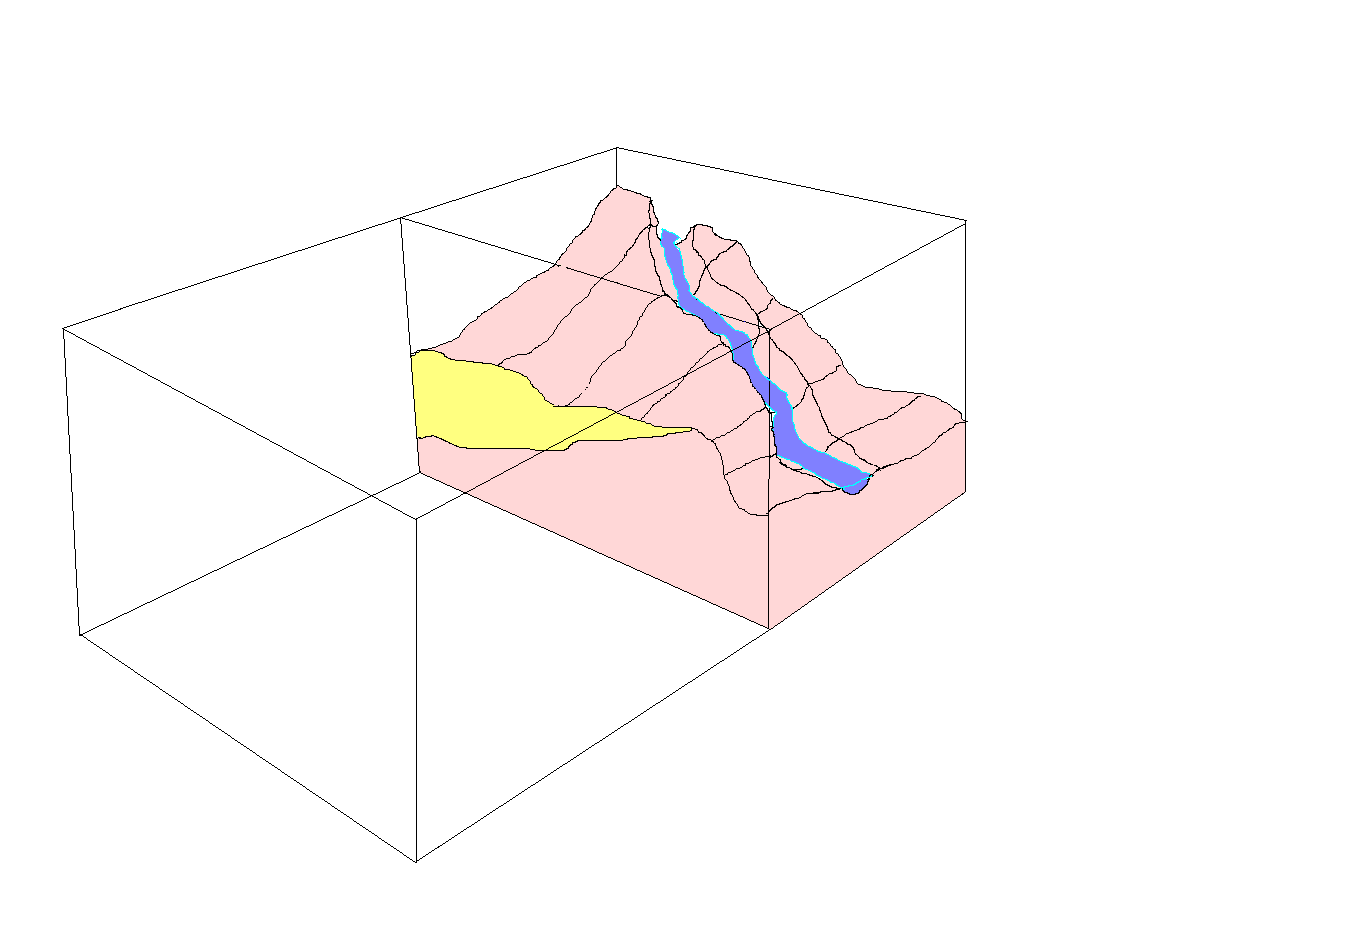
\includegraphics[width=4in]{newCube}
\caption[]{
  \footnotesize
  Now we might add a new cube to expand our drawing
  \label{fig:newCube}
}
\end{figure}

\begin{figure}
\centering
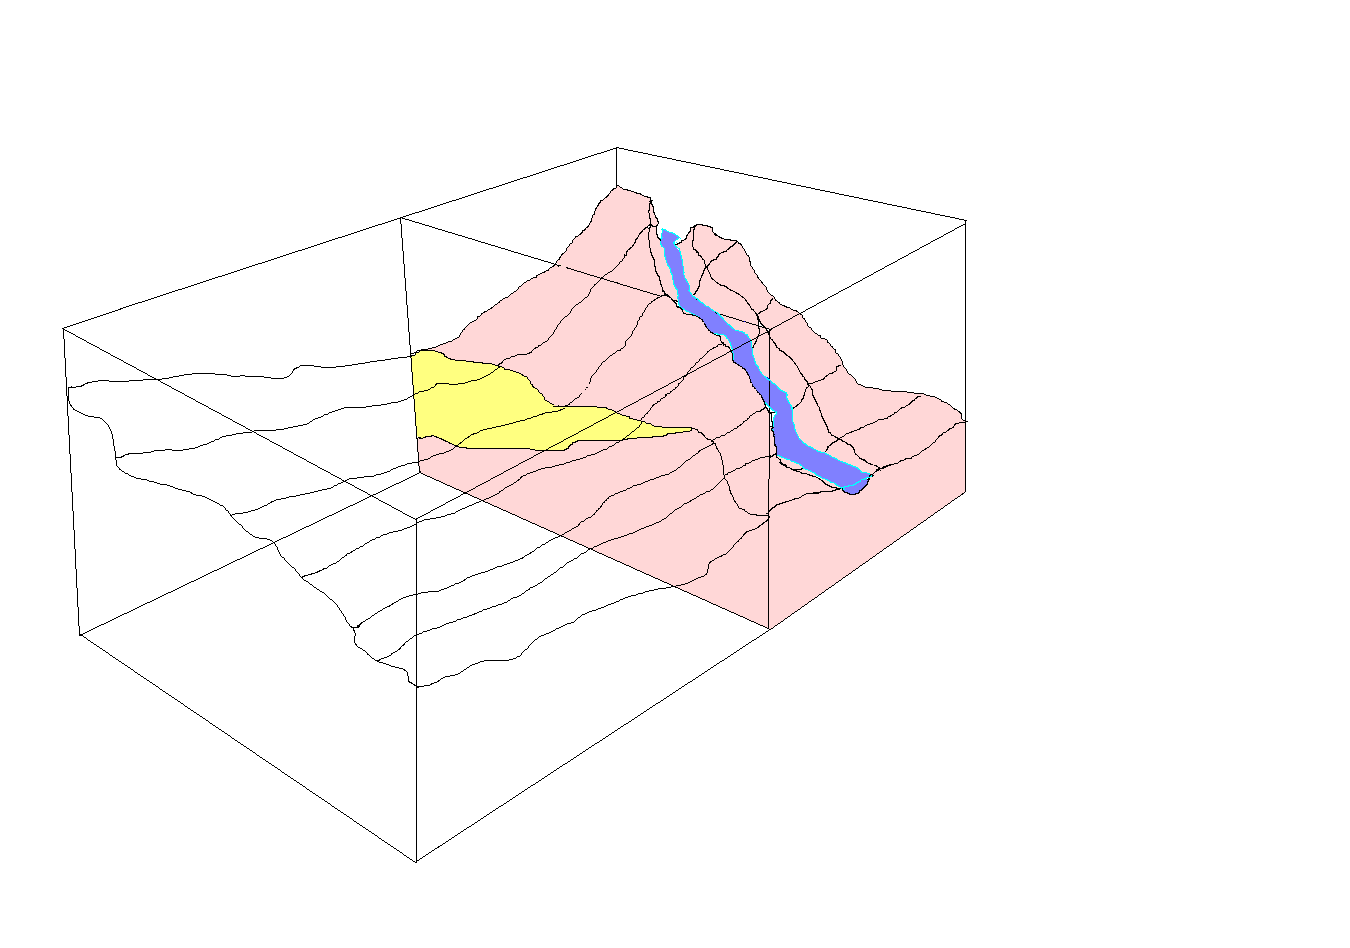
\includegraphics[width=4in]{newCubeLayer}
\caption[]{
  \footnotesize
  Drawing a new layer. Lines snap towards existing lines in adjacent cube.
  \label{fig:newCubeLayer}
}
\end{figure}

\begin{figure}
\centering
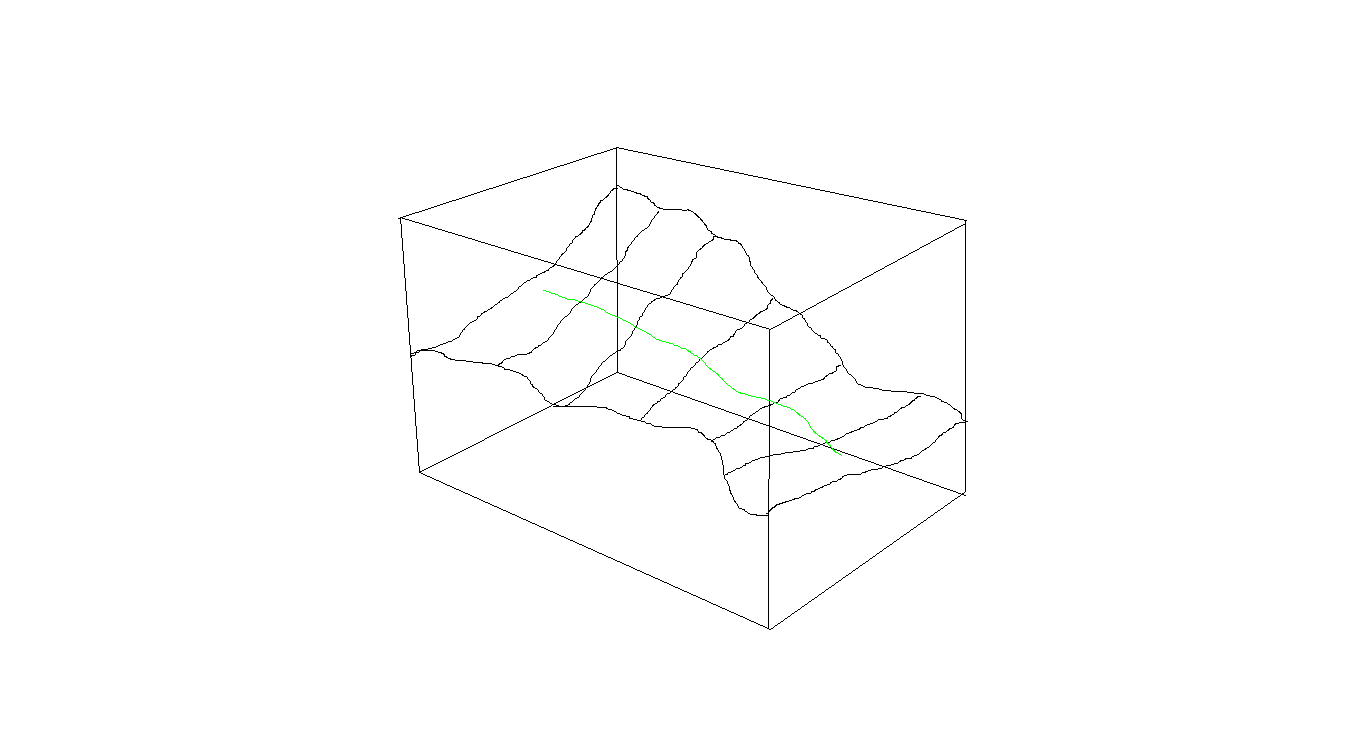
\includegraphics[width=4in]{createRidge0}
\caption[]{
  \footnotesize
  To create a new ridge or valley, start by drawing the ridge or valley path on the existing terrain. 
  \label{fig:createRidge0}
}
\end{figure}

\begin{figure}
\centering
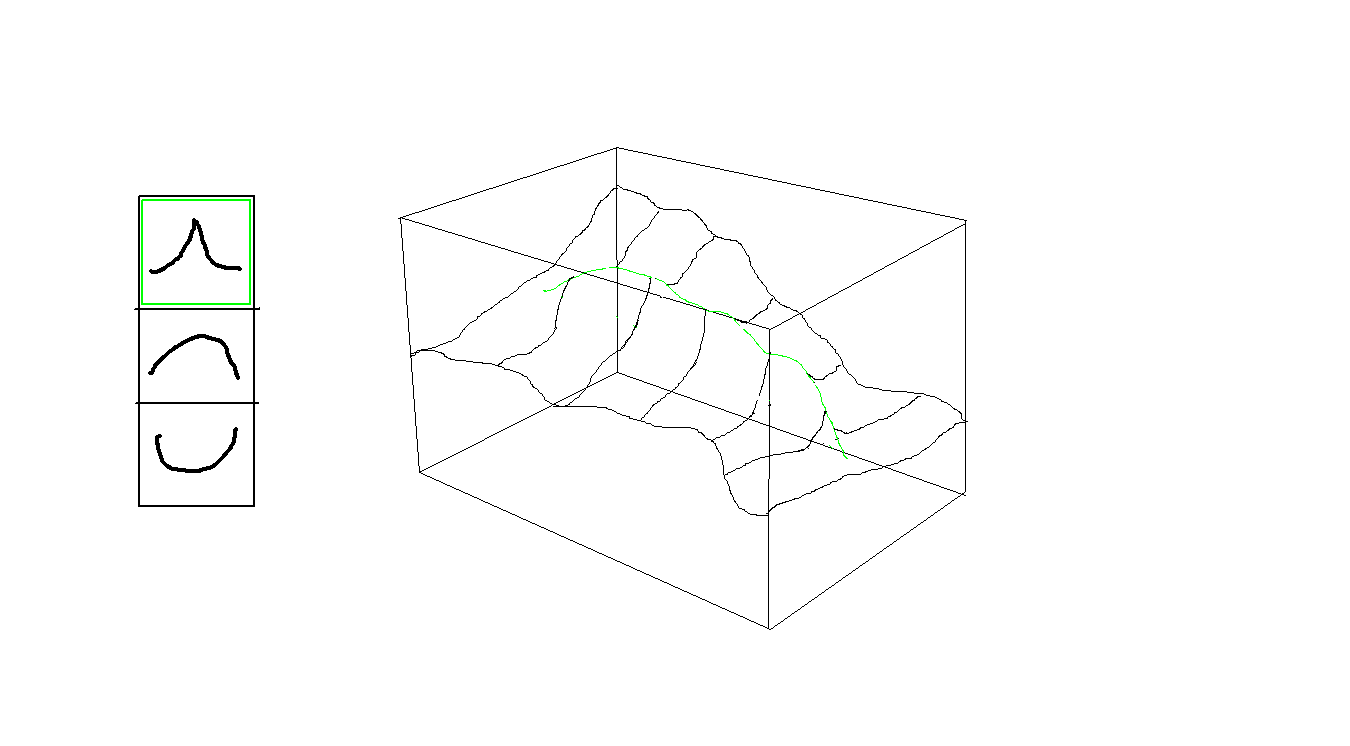
\includegraphics[width=4in]{createRidge1}
\caption[]{
  \footnotesize
  Now chose what the contour will look like and the new feature will be created. It should be possible to create different contours along different positions on the path drawn. 
  \label{fig:createRidge1}
}
\end{figure}

\clearpage

\section*{Reading list}
\begin{itemize}
 \item Sequence stratigraphy-A global theory for local success, Neal
 \item Interactive thickness visualization of articular cartilage, Mlejnek
\end{itemize}
\end{itemize}


\end{document}

